\section{Nodes}

In the nutshell node is a Linux machine with special software installed.

This software is called \textbf{ORC}, using it \textbf{OCTA CORE} is able to establish secure communication channel to the node.

Communication between \textbf{OCTA CORE} and \textbf{ORC} is doing in RPC\cite{rpc} like manner.

Secure channel is implemented using HTTPS\cite{https} protocol with validating each request using security token.

\begin{figure}[H]
    \centering
    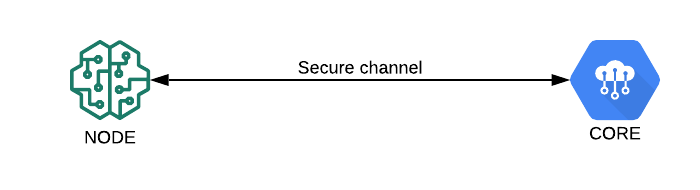
\includegraphics[scale=0.5]{core-orc-channel}
    \caption{Secure communication channel}
\end{figure}

\textbf{ORC} is responsible for the following activities:

\begin{itemize}
    \item Detect installed hardware: CPU, GPUs, RAM, volume of disk storage
    \item Collect metrics about hardware usage, like free/used disk/ram space, CPU and GPU load, temperature and fans speed
    \item Manage Docker\cite{docker} containers and Firecracker\cite{firecracker} microVMs
\end{itemize}

There are two types of nodes: \textbf{blockchain} and \textbf{service}

The first one is responsible for support of OCTA Layer 1 blockchain by running network node software.
As a result such nodes making network more stable, distributed, more latency fair and speed up the synchronization.

Service node provides resources we used to implement services for the end users.

\subsection{Hardware and software requirements}

To cover a wide range of supported hardware, node software can be installed on any machine with x86\_64\cite{x86_64} or ARM\cite{arm} architecture.

In order to run the node, the hardware must meet the minimum system requirements, which are as follows: 1 CPU, 1 Gb of RAM, and 10Gb of free disk space.

However, the requirements for hardware may vary depending on the intended purpose of the node. For instance, a node that provides only VPN services may only need to meet the minimum requirements. Conversely, nodes that are designed to perform AI/ML tasks will require powerful GPUs connected with a high bandwidth PCIe interface, as well as ample disk storage.

It's worth noting that both NVIDIA and AMD GPUs are supported by the system.

To determine the performance of a node, the following measurements are taken:

\begin{itemize}
    \item Network upload/download speed
    \item Disk write speed
    \item GPU performance using AI benchmark (only for NVIDIA)
\end{itemize}

These performance metrics help users to choose the hardware they need for their tasks.

The node software can be installed on any Linux distribution; however, we primarily focus on Ubuntu LTS or Debian as the recommended operating systems.

Support for Windows in development.

\subsection{Security}

To eliminate possible security risks for users running the software \textbf{ORC} on their machines, we follow a set of rules and guidelines, which include: 

\begin{itemize}
    \item \textbf{ORC} is open sourced, this may possible to make audit by other people that software does not have malicious code
    \item Keep code base of \textbf{ORC} is small as possible for ease auditing
    \item Node software run under non privilaged user and don't have any permissions which not need for operation
    \item Regular software updates to ensure that the latest security patches are applied. Along with comprehensive testing of software to detect and address any potential security issues.
\end{itemize}

\subsection{Verification}

Ensuring that node infrastructure operates smoothly and reliably is crucial for providing high-quality services to end-users.

Each new node that joins the cloud must be verified and confirmed to meet the necessary requirements and provide services.

Periodically, we conduct re-verification checks on verified nodes. Therefore, it's crucial to monitor the status of your nodes to avoid having them changed to an unverified status.

The checks performed to ensure that the node is properly configured may include but are not limited to:

\begin{itemize}
    \item Meet minimum hardware requirements
    \item System clock is synchronized
    \item All necessary network ports are open
    \item GPU driver is correctly installed
\end{itemize}

The list of checks will be expanding in the future to ensure even greater accuracy and reliability.

The following restrictions are applied for the unverified nodes:

\begin{itemize}
    \item Nodes can't provide services
    \item Nodes can't participate in \hyperref[sec:staking]{staking}
\end{itemize}
